
\newpage

\section{Model Structure}

\subsection{General Description}

With the data acquired from HuggingFace, the process of making a machine learning model could begin. The model that was developed was a convolutional neural network (CNN). It accepts full-size images of shape $(512, 512, 3)$, with each image being an rgb image with values ranging from 0 to 255. \Cref{code:model_definition} shows the \code{src/model_def.py} file, which was called by the \code{main.ipynb} and \code{src/train.py} files to train and tune the model.

\begin{figure}[h]
    \lstinputlisting[language=Python, caption=Model definition code extract, label=code:model_definition]{code_chunks/sec_3_model.py}
\end{figure}

For the first section, a \code{Conv2D} layer was applied with a kernel size of $3{\times}3$ and a tunable number of filters, $f_{1}$. The stride was fixed at its default value of $1$, with padding set to \emph{same} which preserves the spatial dimensions of the input feature maps, at the cost of increased computational cost. A \code{ReLU} activation function was used due to its simplicity and its ability to address vanishing gradients.

This was followed by a pooling layer, where either max pooling or average pooling could be selected. By default, the pooling operation uses a window of size $2{\times}2$ with stride $2$, reducing the spatial resolution of the feature maps by half while retaining the most salient information.

The second convolutional block repeated this process with a kernel size of $3{\times}3$ and a tunable number of filters, $f_{2}$, again followed by either max or average pooling with window size $2{\times}2$ and stride $2$.

After the two convolutional blocks, a global pooling layer was applied to remove the spatial dimensions, with a max or average pooling being optional. The dense head consisted of a flattening step, followed by a fully connected layer with $d$ units and ReLU activation. An optional dropout layer with rate $p$ was included for regularisation. The final output layer was a single neuron with sigmoid activation, producing a probability for binary classification.

Adam was chosen as one of the considered optimisers, as it is known to converge rapidly, and rectifies vanishing learning rate and high variance, therefore being the most popular optimiser \cite{RAIAAN2024100470}. Adagrad was chosen as the second potential optimiser, as the learning rate would not need manual tuning, and is known to perform better than alternatives like SGD, MBGD, and primitive momentum based optimisers. Though it should be noted that it has the weakness of a constantly decreasing learning rate, resulting in slower convergence \cite{RAIAAN2024100470}

The loss function that was used for this model was binary cross-entropy, as it is the most suitable loss function for binary classification tasks. Each model training instance was trained for 3 epochs, on a \code{ml.c5.2xlarge} instance type, favoring low cost over time efficiency.

\newpage

\subsection{Hyperparameter Tuning with Hyperband}

Hyperparameter tuning was performed to maximise the models performance through iteration of most of its parameters. The hyperparamter tuning process was performed on the small train set, for faster iteration.

\Cref{tab:tunable_hyperparameters}, summarises the code snippets seen in \cref{code:hyperparameter_tuning}, depicting a list of the parameters being tuned in the above model, as well as the final value that the tuner settled on. It is evident that this was a very large parameter space, and it is therefore not feasible to find the best possible hyperparamer using a simple grid search. Instead, the Hyperband algorithm was used to tune the hyperparameters, as it is a bandit-based algorithm that uses early stopping to focus on the most promising hyperparameter combinations \cite{hyperband}.

Following the initial tuning on the smaller dataset, the best hyperparameters were selected and used to train the model on the larger training set, the start of this can be seen in \cref{code:hyperparameter_extraction}

\begin{table}[h]
    \centering
    \caption{Tunable Hyperparameters and Final Chosen Values (see implementation snippets in \cref{code:hyperparameter_tuning})}
    \begin{tabular}{lll}
    \toprule
    \textbf{Hyperparameter} & \textbf{Range/Choices} & \textbf{Final Value} \\
    \midrule
    learning rate           & $1{\times}10^{-4}$ to $1{\times}10^{-2}$ (log scale) & 0.00149 \\
    dropout-rate            & $0.0$ to $0.5$ (used if \texttt{use-dropout=true}) & 0.284 \\
    conv1-filters ($f_1$)   & $16$ to $128$ & 24 \\
    conv2-filters ($f_2$)   & $32$ to $256$ & 107 \\
    dense-units ($d$)       & $64$ to $512$ & 254 \\
    pooling                 & \texttt{max}, \texttt{avg} & max \\
    use-dropout             & \texttt{true}, \texttt{false} & true \\
    optimizer               & \texttt{adam}, \texttt{adagrad} & adam \\
    \bottomrule
    \end{tabular}
    \label{tab:tunable_hyperparameters}
\end{table}

\begin{figure}[h]
    \lstinputlisting[language=Python, caption=Hyperparameter extraction code snippet, label=code:hyperparameter_extraction]{code_chunks/sec_3_hp_extraction.py}
\end{figure}

\begin{figure}[p]
    \lstinputlisting[language=Python, caption=Hyperparameter tuning code extracts from \code{main.ipynb} and \code{src/train.py}; used to call \code{src/model_def.py} (\cref{code:model_definition}), label=code:hyperparameter_tuning]{code_chunks/sec_3_hp_tuning.py}
\end{figure}

\newpage

\section{Model Deployment} \label{sec:model_deployment}

This model, along with the transfer learning model described in \cref{sec:transfer_learning}, was deployed using Amazon SageMaker, as shown in \cref{fig:endpoint}. The deployment code is provided in \cref{code:deployment_endpoint}, which includes exception handling to initialise the \code{main_model_predictor} only if it is not already in memory. \Cref{code:deployment_endpoint} also includes the inference logic used to generate predictions on the holdout set. Further discussion of the deployment process and associated challenges is provided in the AWS reflection section (\cref{sec:model_deployment}).

\begin{figure}[h]
    \centering
    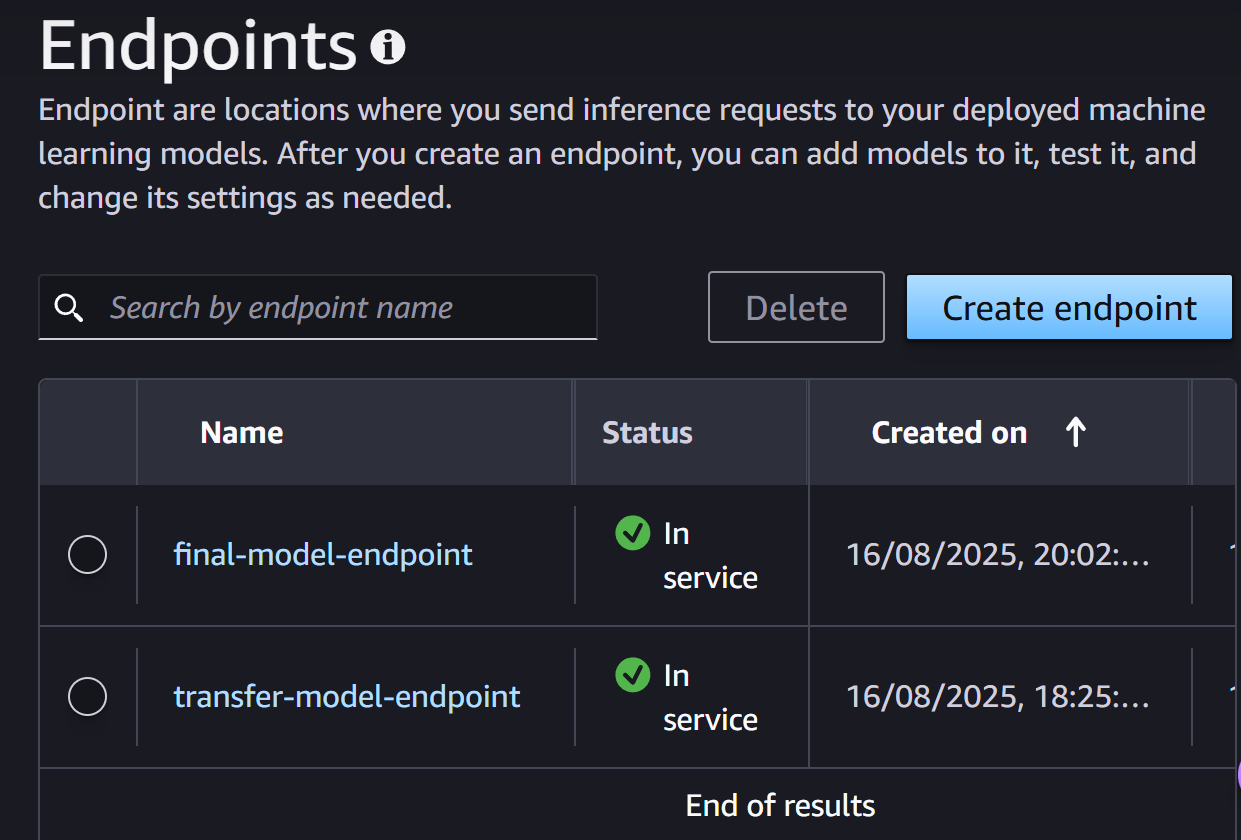
\includegraphics[width=200px]{figures/endpoints_screenshot.png} % Image filename
    \centering
    \caption{Endpoint page screenshot in Sagemaker, as evidence of deployment} % Caption
    \label{fig:endpoint} % Label
\end{figure}

\begin{figure}[h]
    \lstinputlisting[language=Python, caption=Model Deployment and inference code snippet, label=code:deployment_endpoint]{code_chunks/sec_4_example_deployment.py}    
\end{figure}

\newpage

\section{Transfer Learning} \label{sec:transfer_learning}

Several CNN architectures are available for transfer learning, as outlined in \cite{keras_applications}. EfficientNetV2 was selected due to its demonstrated balance between accuracy and computational efficiency on general image classification tasks, making it suitable for the diverse image content in the aiornot dataset \cite{keras_applications, tan2021efficientnetv2}.

EfficientNetB0, pre-trained on ImageNet, was used as a feature extractor with its classification head removed and average pooling applied. The final 10\% of layers were unfrozen to enable fine-tuning. A dropout layer with rate $p$ was included for regularisation, followed by a dense output layer with sigmoid activation to produce a binary class probability. The model accepted inputs of shapes that were smaller than the original 500x500 due to issues with memory allocation during training. The \code{src/transfer_learning.py} script defined the model and training logic, and was invoked by the \code{transfer_learning.ipynb} notebook; selected code snippets are shown in \cref{code:transfer_learning_code}.


\begin{figure}[h]
    \lstinputlisting[language=Python, caption=Transfer Learning Code Snippet, label=code:transfer_learning_code]{code_chunks/sec_5_transfer_learning.py}
    \label{fig:transfer_learning_code}
\end{figure}

The model was then deployed to a SageMaker endpoint using the same strategy shown previously in \cref{code:deployment_endpoint}, and evaluated on precision, recall, F1 score, and accuracy.

\newpage

\section{Model Comparison And Evaluation}

In this section, we compare the performance of the different models trained on the dataset. Evaluation metrics were calculated by invoking the model endpoints on the holdout set, which was not used during training or validation. This ensures that the models' performance is on unseen data, better modelling a general use case.

\begin{table}[h]
\centering
\caption{Model Comparison}
\begin{tabular}{rcccc}
\toprule
\textbf{Model} & \textbf{Accuracy} & \textbf{Precision} & \textbf{Recall} & \textbf{F1 Score} \\
\midrule
Main Model     & 0.854          & 0.833          & \textbf{0.906} & \textbf{0.868} \\
Transfer Model & \textbf{0.856} & \textbf{0.875} & 0.849 & 0.862 \\
\midrule
$\text{abs}(\text{Difference}) $ & 0.002 & 0.042 & 0.057 & 0.006 \\
\bottomrule
\end{tabular}
\label{tab:model_comparison}
\end{table}

\begin{figure}[h]
    \centering
    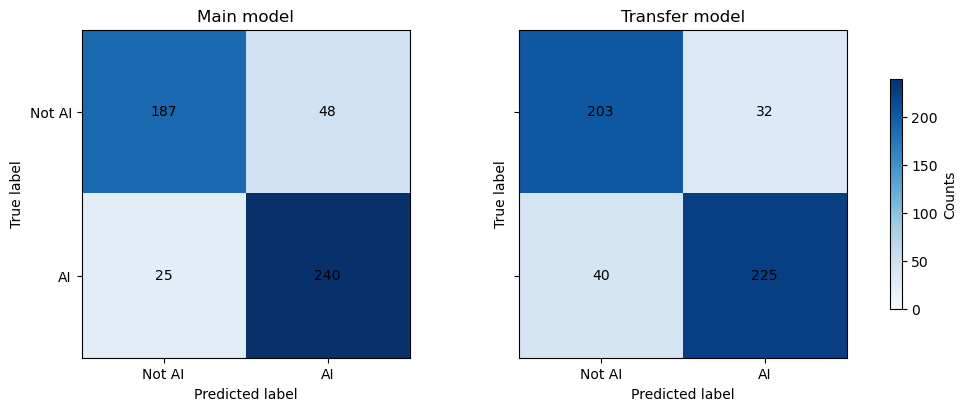
\includegraphics[width=0.8\linewidth]{figures/confusion_matrix.png} % Image filename
    \centering
    \caption{Confusion Matrix of main model and transfer learning model} % Caption
    \label{fig:confusion_matrixes} % Label
\end{figure}

The results of the model evaluation are summarized in \Cref{tab:model_comparison}. The table highlights the key performance indicators for each model. It can be seen that the EfficientNet transfer learning model and the main model have very comparable performance - with the EfficientNet model and main model achieving an accuracy of 85.6\% and 85.4\% respectively - a difference of only 0.2\%. Furthermore the EfficientNet and main model achieved F1 scores of 0.862 and 0.868 respectively, a difference of only 0.006.

Where these models differ is their precision and recall. The EfficientNet model achieved a precision of 87.5\% (4.2\% higher than the main models' 83.3\%.) The main model achieved a recall of 90.6\% (5.7\% higher than the EfficientNet models' 84.9\%.) This means that the EfficientNet model is better at minimising false positive AI detection, whereas the main model is better at detecting AI cases without missing them (i.e. reducing false negatives). This is evident in \cref{fig:confusion_matrixes}, where the EfficientNet model has 32 false posiives compared to the main models' 48. Similarly, the main model has only 25 false negatives, compared to the EfficientNet models' 40.

\newpage

\section{AWS Sagemaker Information and Discussion} \label{sec:aws_reflection}

This project was developed using AWS SageMaker. \Cref{fig:jupyter_lab_space_config} shows the JupyterLab environment configuration used. The smallest available instance type, \code{ml.t3.medium}, was selected for the notebook environment, as model training was offloaded to separate training jobs with dedicated compute resources. Each training job used the \code{ml.c5.2xlarge} instance type, chosen for its higher RAM and CPU availability.

\Cref{fig:file_top,fig:file_src} shows the file structure used in the project, as run within the JupyterLab environment. The model definition code (\code{src/model_def.py} and \code{src/transfer_model.py}) and the training scripts (\code{src/train.py} and \code{src/train_transfer.py}) were separated from the main notebooks to improve modularity and reusibility for any case where another notebook would need to call upon these models' structure.


\begin{figure}[h]
    \centering
    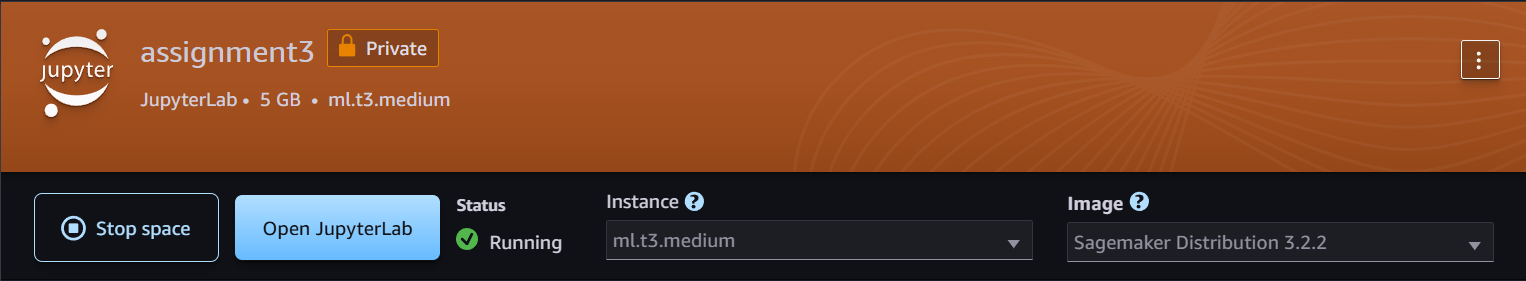
\includegraphics[width=0.8\linewidth]{figures/jupyter_lab_space_config.png} % Image filename
    \centering
    \caption{Jupyter lab space configuration screenshot} % Caption
    \label{fig:jupyter_lab_space_config} % Label
\end{figure}

\begin{figure}[htbp]
    \centering
    \begin{minipage}{0.3\textwidth}
        \centering
        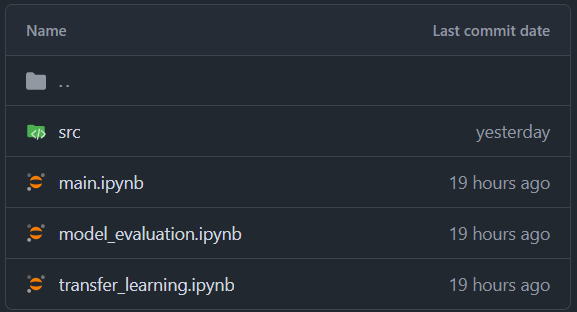
\includegraphics[width=\linewidth]{figures/file_structure_top.png}
        \caption{Top level file structure screenshot}
        \label{fig:file_top}
    \end{minipage}\hfill
    \begin{minipage}{0.3\textwidth}
        \centering
        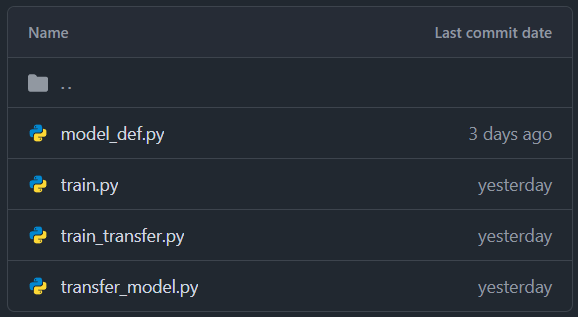
\includegraphics[width=\linewidth]{figures/file_structure_src.png}
        \caption{Files inside the \code{src} directory screenshot}
        \label{fig:file_src}
    \end{minipage}\hfill
    \begin{minipage}{0.35\textwidth}
        \centering
        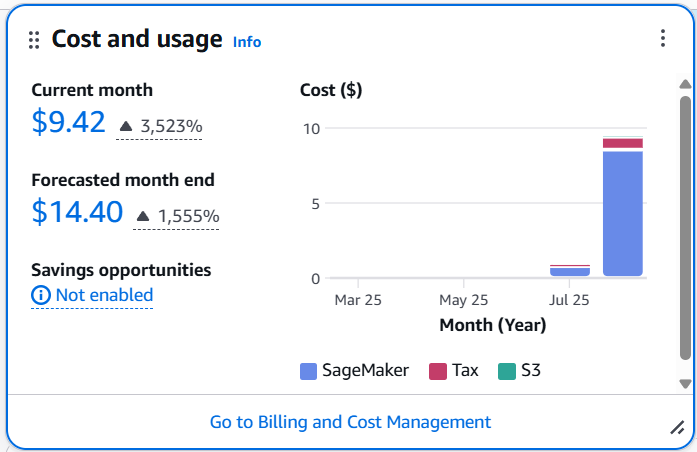
\includegraphics[width=\linewidth]{figures/aws_cost_summary.png} % Image filename
        \caption{Project AWS cost summary screenshot} % Caption
        \label{fig:aws_cost_summary} % Label
    \end{minipage}\hfill
\end{figure}


\Cref{fig:aws_cost_summary} shows the total cost summary for the project, which remained under \$15. This was achieved through careful resource management within a known budget of \$50. General-purpose \code{ml.c5.2xlarge} instances were selected for both training and inference, avoiding more expensive GPU backed instances. While GPU instances would have significantly reduced training time due to their parallel computing capabilities, well suited to machine learning workloads the increased cost was not justified within the project constraints. This tradeoff resulted in longer training times but was acceptable given the budget, and the workflow remains easily extensible to a GPU-backed configuration in a real world deployment. The main model took 56 minutes to train, while the transfer learning model required 67 minutes. Both were trained for 3 epochs on the same \code{ml.c5.2xlarge} instance type.

An issue encountered during the project was related to model deployment. Specifically, the models were deployed as real time endpoints, operating on a server and accessed via HTTP requests. While this allowed the endpoints to be invoked at any time by users with appropriate permissions, it also imposed a payload limit, restricting each request to a maximum of four $500 \times 500$ RGB images. This made the evaluation process slower. As a result, the holdout set was limited to 500 images, since the evaluation workflow was not scalable. Due to limited experience with AWS, configuring a more appropriate batch inference or transformer endpoint proved difficult, and the real time endpoint was used as a compromise.

Due to limited experience with SageMaker and a highly cost conscious mentality, memory issues were encountered during training of the transfer learning model. As a result, the following compromises were made:
\begin{itemize}
    \item reducing the batch size of the transfer learning model,
    \item downsampling images to a resolution of $224 \times 224$,
    \item selecting the EfficientNetB0 architecture instead of higher-capacity alternatives such as EfficientNetB1 or EfficientNetB2.
\end{itemize}
these issues could be very easily addressed with more resources, particularly given that the way in which the model definition code and training scripts were structured in a modular way.


\section{Final Model Discussion and Conclusion}

This report proposed two models to detect if an image is generated using ai - one model developed through hyperparameter tuning, and the other through transfer learning from EfficientNet. The results indicate that both models perform comparably, with slight differences in precision and recall.

The original research objective was to make a tool to distinguish between AI-generated and real images, ultimately as a means to identify the spread of misinformation and other harms in online discourse. Were this model to be deployed as a 'first step' with the intention of more thoughrough investigation, it would be more beneficial to be relaxed on false positives, and minimise false negatives, given the false positives would be vindicated with further analysis or research.

For this reason, under the current configuration, the main model is the preferred option, as it achieves a higher recall (90.6\% vs 84.9\%) and is therefore slightly better at detecting AI-generated images without missing them. However, as discussed in \cref{sec:aws_reflection}, with increased resources, the transfer learning model could be trained at full resolution using a higher capacity architecture such as EfficientNetB2. This would likely improve its performance further, surpassing the main model in both precision and recall, given that it performs comparably even under the current constraints.

While this project achieved comparable accuracy (85.4\% and 85.6\% on the main and transfer learning models respectively) to that reported in \cite{bird2023cifakeimageclassificationexplainable}, which reached nearly 93\% using CNNs and the CIFAKE dataset, it is important to acknowledge that the performance demonstrated here does not reflect research-level rigour. The CIFAKE dataset introduced in that study is a large and diverse benchmark designed to support broader generalisation and deeper analysis across model types. Due to limited experience and project constraints, this dataset was not fully utilised, and evaluation was instead conducted on a smaller, custom-generated holdout set. As such, while the results achieved in this project are competitive within scope, further development would be required to ensure a proper comparison with comparable approaches in the literature.

Overall, it can be concluded that the models developed in this investigation are effective at distinguishing AI-generated images from real ones, with two models successfully trained and deployed to perform this task.
